\documentclass[12pt]{article}
\usepackage{times} 			% use Times New Roman font

\usepackage[margin=1in]{geometry}   % sets 1 inch margins on all sides
\usepackage[hidelinks]{hyperref}               % for URL formatting
\usepackage[pdftex]{graphicx}       % So includegraphics will work
\setlength{\parskip}{1em}           % skip 1em between paragraphs
\usepackage{indentfirst}            % indent the first line of each paragraph
\usepackage{datetime}
\usepackage[small, bf]{caption}
\usepackage{listings}               % for code listings
\usepackage{xcolor}                 % for styling code
\usepackage{multirow}

%New colors defined below
\definecolor{backcolour}{RGB}{246, 246, 246}   % 0xF6, 0xF6, 0xF6
\definecolor{codegreen}{RGB}{16, 124, 2}       % 0x10, 0x7C, 0x02
\definecolor{codepurple}{RGB}{170, 0, 217}     % 0xAA, 0x00, 0xD9
\definecolor{codered}{RGB}{154, 0, 18}         % 0x9A, 0x00, 0x12

%Code listing style named "gcolabstyle" - matches Google Colab
\lstdefinestyle{gcolabstyle}{
  basicstyle=\ttfamily\small,
  backgroundcolor=\color{backcolour},   
  commentstyle=\itshape\color{codegreen},
  keywordstyle=\color{codepurple},
  stringstyle=\color{codered},
  numberstyle=\ttfamily\footnotesize\color{darkgray}, 
  breakatwhitespace=false,         
  breaklines=true,                 
  captionpos=b,                    
  keepspaces=true,                 
  numbers=left,                    
  numbersep=5pt,                  
  showspaces=false,                
  showstringspaces=false,
  showtabs=false,                  
  tabsize=2
}

\lstset{style=gcolabstyle}      %set gcolabstyle code listing

% to make long URIs break nicely
\makeatletter
\g@addto@macro{\UrlBreaks}{\UrlOrds}
\makeatother

% for fancy page headings
\usepackage{fancyhdr}
\setlength{\headheight}{13.6pt} % to remove fancyhdr warning
\pagestyle{fancy}
\fancyhf{}
\rhead{\small \thepage}
\lhead{\small HW\#2, Huang}  % EDIT THIS, REPLACE # with HW number
\chead{\small DATA 440, Fall 2022} 

%-------------------------------------------------------------------------
\begin{document}

% EDIT THE ITEMS HERE
\begin{centering}
{\large\textbf{Archiving the Web}}\\ 
Sofia Huang\\
due 10/11/2022\\
\end{centering}

%-------------------------------------------------------------------------

% The * after \section just says to not number the sections
\section*{1. Collect URIs from Tweets}
\noindent \textbf{\begin{itemize}
\item Write a Python program that collects English-language tweets that contain links. 
\item Write a Python program that extracts the links shared in tweets.
\item Resolve all URIs to their final target URI (i.e., the one that responds with a 200).
\item Save only unique final URIs (no repeats).
\item if after this step, you don't have 1000 unique URIs, go back and gather more until you are able to get at least 1000 unique URIs
\item Save this collection of 1000 unique links in a file and upload it to your repo in GitHub
\end{itemize}}

I used the function from get\_tweets.py from a previous homework to collect 12,500 English tweets using the keywords: `Queen’, `hurricane’, `Ukraine’, `NASA’, and `Biden’. Then, I read the JSONL file, one line at a time, to obtain any links from each tweet. I also used regex to check if the link led to a Twitter page or any video/audio only site and did not store those links. I also used the requests library to resolve links to their final URI and stored them all in a .txt file. I ended up with 16,004 resolved links. 


\begin{lstlisting}[language=Python, caption=Collecting tweets and extracting links, label=lst:copy]
import sys
import json
from twarc import Twarc2, expansions
from configparser import ConfigParser
import re
from subprocess import call
import requests
import os
import time
import csv

TWARC_CONFIG_FILE = "/Users/sofiahuang/Library/Application Support/twarc/config"
OUTPUT_FILE = "/Users/sofiahuang/Documents/WM/FALL2022/DATA440/tweets.jsonl"   # line-oriented JSON
MAX_TWEETS = 100

def get_tweets(input_search_term):
    # read Twitter API keys from twarc config file, setup twarc2 object
    config = ConfigParser(interpolation=None)
    with open(TWARC_CONFIG_FILE) as twarc_config:
        config.read_string("[TWARC]\n" + twarc_config.read())
    bearer_token = config['TWARC']['bearer_token'].strip('\'')
    t = Twarc2(bearer_token=bearer_token)

    search_term = input_search_term

    # limit search results to English language, with links, and no retweets
    query = search_term + " lang:en has:links -is:retweet"

    search_results = t.search_recent(query=query, max_results=MAX_TWEETS)
    # max_results is the number of results per page

    num_tweets = 0
    for page in search_results:
    # use expansions.flatten to get all the information in a single JSON
        result = expansions.flatten(page)

    # open the file and write one JSON object per new line (jsonl format)
        with open(OUTPUT_FILE, 'a+') as filehandle:   # if you want to append, change 'w' to 'a+'
            for tweet in result:
                print(tweet)
                filehandle.write('%s\n' % json.dumps(tweet))
                num_tweets = num_tweets + 1
                if num_tweets == MAX_TWEETS:
                # must include this to stop after a certain # of tweets
                    search_results.close()

    print (num_tweets, "tweets written to " + OUTPUT_FILE + " for query \"" + query + "\"\n");

def get_links():
    f = open(OUTPUT_FILE)
    # read in all the lines
    lines = f.readlines()  
    links = []
    resolved_links = []
    # each line is a json 
    for line in lines:
        tweet_data = json.loads(line) 
        # collect links 
        if 'urls' in tweet_data['entities']:
            for link in tweet_data['entities']['urls']:
                # check if link leads to a Twitter or video/audio only page using regex
                pattern = re.compile('(https:\/\/)(www\.|.*)(twitter|youtube|youtu|tiktok|twitch|soundcloud)(\.com|\.be)(.*)')
                m = pattern.match(link['expanded_url'])
                if (m == None):
                    # add to list if link leads to an acceptable page (not Twitter or video/audio)
                    links.append(link['expanded_url'])
                    #print('original: ' + link['expanded_url'])
                    try:
                        # resolve links to their final URI
                        resolved_link = requests.head(link['expanded_url'], allow_redirects=True, timeout=5).url
                        resolved_links.append(resolved_link)
                        #print('final: ' + resolved_link)
                    except:
                        continue
    print('Originally ' + str(len(links)) + ' links.')
    print('Resolved ' + str(len(resolved_links)) + ' links.')
    os.chdir("/Users/sofiahuang/Documents/WM/FALL2022/DATA440")
    # create txt file to store the resolved links
    resolved_uri_file = os.path.join(os.getcwd(), 'resolved_uris.txt')
    for link in resolved_links:
        try:
            with open(resolved_uri_file, 'a+') as f:
                f.write("\n%s" % link)
                print(link)
        except Exception as e:
            print(e)
    return resolved_links
\end{lstlisting}

\begin{lstlisting}[language=Python, caption=Running get\_tweets() and get_links(), label=lst:copy]
if __name__ == "__main__":
    search_terms = ['Queen', 'hurricane', 'Ukraine', 'NASA', 'Biden']
    for term in search_terms:
        for i in range(25):
            get_tweets(term)

    final_links = get_links()
\end{lstlisting}


Then, I used the Unix tools, sort and uniq to save only the unique URIs from resolved\_uris.txt to a seperate .txt file. I ended up with 2,146 unique URIs stored.

\begin{lstlisting}[language=bash, caption=Keeping only unique URIs, label=lst:copy]
(base) sofiahuang@Sofias-MacBook-Pro DATA440 % sort resolved_uris.txt | uniq > unique_uris.txt 
(base) sofiahuang@Sofias-MacBook-Pro DATA440 % wc -l unique_uris.txt
    2146 unique_uris.txt
\end{lstlisting}


\section*{2. Get TimeMaps for Each URI}
\noindent \textbf{Obtain the TimeMaps for each of the unique URIs from Q1 using the ODU Memento Aggregator, MemGator.}

I read the .txt file with the unique URIs into a list and created a function to run MemGator, locally,  on each of the URIs. I stored the timemaps I obtained in folder and ended up with 1,072 timemaps. I was unable to get timemaps for all of the unique URIs I had stored and I believe this has something to do with the MemGator server and maybe it didn't work for all of them.

\begin{lstlisting}[language=Python, caption=MemGator to get timemaps for all unique URIs, label=lst:copy]
def read_unique_links_file(txt_filename):
    # check if we are in the correct directory
    os.chdir("/Users/sofiahuang/Documents/WM/FALL2022/DATA440")
    summary_filename = os.path.join(os.getcwd(), txt_filename)
    # read the resolved links txt file into a list to be returned
    try:
        summary_file = open(summary_filename, 'r')
        url_data = summary_file.read()
        unique_list = url_data.split("\n")
        summary_file.close()
        print(str(len(unique_list)))
        return unique_list
    except Exception as e:
        print(e)
        return []

def get_timemaps(list, directory):
    # to keep track of how many URIs timemaps are obtained for
    # and to name the timemaps json file returned from MemGator
    link_index = 1
    for uri in list:
        filename = str(link_index) + ".json"
        # create a folder to store the timemaps
        if os.path.exists(os.path.join(directory, filename)):
            # file has already been created, just increment index and go to the next file
            print("Skipping url " + uri + ", file already exists")
            link_index += 1
            continue
        else:
            # run MemGator on each URI in the unique links list
            print('running memgator on: ' + uri)
            time.sleep(1)
            os.system('/Users/sofiahuang/Downloads/memgator-darwin-amd64 -F 2 -f JSON ' + uri + ' > /Users/sofiahuang/Documents/WM/FALL2022/DATA440/timemaps/' + filename)
            time.sleep(2)
\end{lstlisting}

\begin{lstlisting}[language=Python, caption=Running functions to get timemaps for the URIs, label=lst:copy]
if __name__ == "__main__":
    # ...more function calls before, shown in previous question
    links = read_unique_links_file('unique_uris.txt')
    os.chdir("/Users/sofiahuang/Documents/WM/FALL2022/DATA440")
    timemap_directory = os.path.join(os.getcwd(),'timemaps')
    if not os.path.exists(timemap_directory):
        os.mkdir(timemap_directory)
    get_timemaps(links, timemap_directory)
\end{lstlisting}

\section*{3. Analyze Mementos Per URI-R}

\noindent \textbf{Use the TimeMaps you saved in Q2 to analyze how well the URIs you collected in Q1 are archived. Create a table showing how many URI-Rs have certain number of mementos.}

To store the number of mementos for each URI, I created a dictionary. I iterated through all of the timemap json files in the directory and got the number of mementos archived for each URI. If the json file was zero bytes, it had 0 mementos and I stored that information in the dictionary but did not try to read the file as this would cause an error. I then saved this dictionary as a .csv file so I could easily see the data obtained.

\begin{lstlisting}[language=Python, caption=Find how many mementos obtained from each URI and save to CSV file, label=lst:copy]
def read_json():
    # create dictionary and add entry for URI-Rs with 0 mementos
    mem_dict = {0:0}
    os.chdir("/Users/sofiahuang/Documents/WM/FALL2022/DATA440/timemaps")
    file_count = 0
    # iterate over json files
    for json_file in os.listdir("/Users/sofiahuang/Documents/WM/FALL2022/DATA440/timemaps"):
        # open json file
        f = open(json_file, 'r')
        if (json_file == '.DS_Store'):
            continue
        # if file is 0 bytes, don't read, just add data to dictionary
        if (os.stat(json_file).st_size == 0):
            current_val = mem_dict.get(0)
            mem_dict.update({0: current_val+1})
            file_count+=1
            continue
        # read json file
        data = json.loads(f.read())
        # get number of mementos and add to dictionary, 
        # checking if key is already in the dictionary
        mementos = data['mementos']['list']
        mem_count = len(mementos)
        if mem_count in mem_dict:
            current_val = mem_dict.get(mem_count)
            mem_dict.update({mem_count: current_val+1})
        else:
            mem_dict.update({mem_count: 1})
        f.close()
        file_count+=1
        print(file_count)

    # open file for writing dictionary to csv file
    w = csv.writer(open("/Users/sofiahuang/Documents/WM/FALL2022/DATA440/memento_counts.csv", "w"))
    # loop over dictionary keys and values
    for key, val in mem_dict.items():
        # write every key and value to file
        w.writerow([key, val])

\end{lstlisting}

I created a table to show how many URIs had a certain number of mementos. We can see that the majority had 100 or less mementos archived, with 449 URIs having 0. The number drastically decreases as the number of mementos increases. With less than 50 URIs having from 101-1000 mementos. I had 12 URIs that had over 1000 mementos archived, with memento counts ranging from 1,273 to 156,369. I checked to see what webpage had the highest number of mementos and it was a dailymail.co/uk webpage from 1998.

\begin{center}
\begin{tabular}{ |c|c|c| } 
 \hline
 \textbf{Mementos} & \textbf{URI-Rs} \\ 
  \hline
 0 & 449\\ 
  \hline
 1-100 & 568\\ 
 \hline
 101-200 & 17\\ 
 \hline
 201-300 & 11\\ 
 \hline
 301-400 & 7\\ 
 \hline
 401-500 & 0\\ 
 \hline
 501-600 & 2\\ 
 \hline
 601-700 & 2\\ 
 \hline
 701-800 & 0\\ 
 \hline
 801-900 & 1\\ 
 \hline
 901-1000 & 3\\ 
 \hline
 $>$ 1000 & 12\\ 
 \hline
\end{tabular}
\end{center}



\section*{4. Analyze Datetimes of Mementos}
\noindent \textbf{For each of the URI-Rs from Q3 that had $>$ 0 mementos, create a scatterplot with the age of each URI-R} \lstinline{(today - earliest memento datetime)} \textbf{on the x-axis and number of mementos for that URI-R on the y-axis. }

Figure \ref{fig:scattergraph} shows the age and number of mementos for each URI-R.
\begin{figure}[h]
    \centering
    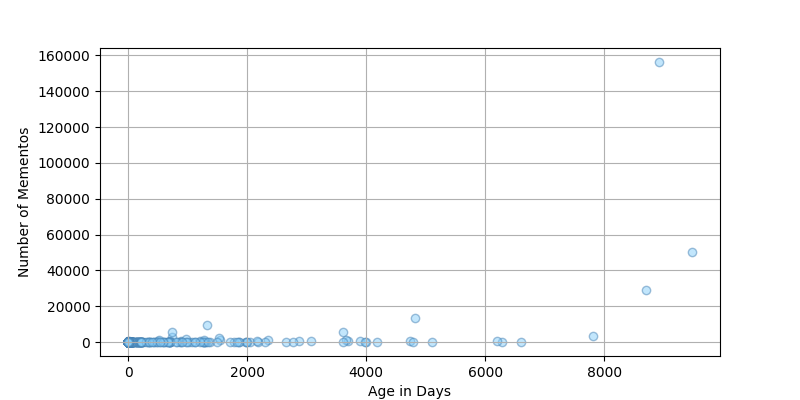
\includegraphics[[width=\textwidth, scale=0.8] {memento_age_scatter.png}
    \caption{Age vs Memento Counts for URI-Rs}
    \label{fig:scattergraph}
\end{figure}

Figure \ref{fig:graph} shows the age and number of mementos for each URI-R without outliers.
\begin{figure}[h]
    \centering
    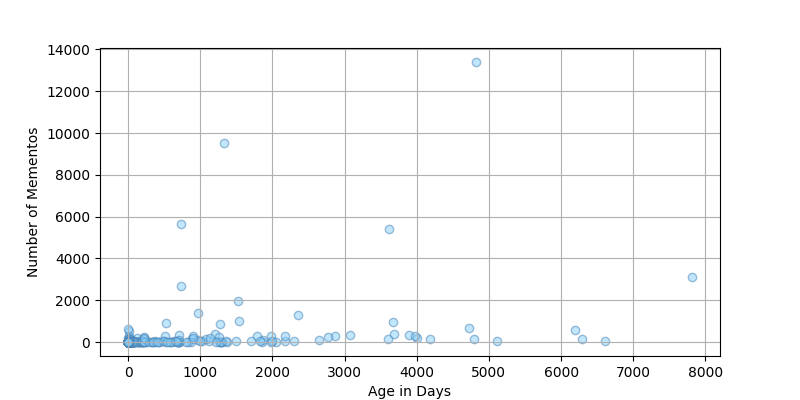
\includegraphics[[width=\textwidth, scale=0.8] {memento_age_scatter_no_outlier.png}
    \caption{Age vs Memento Counts for URI-Rs *excluding URI-Rs with more than 20,000 mementos*}
    \label{fig:graph}
\end{figure}


I iterated through the memento json files and stored the age (using the datetime library), memento count, and URI-R in lists for each URI-R. I created a dataframe out of the 3 lists and then stored the dataframe as a .csv file. Then, I wrote another function to create a scatterplot (using Matplotlib). After I looked at the resulting scatterplot, I decided to create another one without the outliers or the URI-Rs that had greater than 20,000 mementos so that the relationship between age and memento count could be seen more clearly for the lower values.


\textbf{Q: What can you say about the relationship between the age of a URI-R and the number of its mementos?}

Typically, the older URI-Rs have more mementos than newer ones, however the correlation isn't very strong and there are certainly a few outliers. Most of the URI-Rs were only a couple of years old and had less than 1,000 mementos. I included a scatterplot of the same data just excluding the URI-Rs that had over 20,000 mementos so you could see the majority of the data better.

\textbf{Q: What URI-R had the oldest memento? Did that surprise you?}

The URI-R with the oldest memento was 'http://archive.md/19961101130030/http://www.redcross.org/' and it was 9,471 days old or almost 26 years old. The Red Cross has been around for a long time and is a well-known organization so it doesn't surprise me that their webpage has been archived well. 

\textbf{Q: How many URI-Rs had an age of $<$ 1 week, meaning that their first memento was captured the same week you collected the data?}

175 URI-Rs had an age of less than a week. I looked at the .csv file to figure this out.

\begin{lstlisting}[language=Python, caption=Create scatterplot to show age of mementos, label=lst:copy]
def get_memento_age():
    # create dictionary and add entry for URI-Rs with 0 mementos
    mem_dict = {0:0}
    os.chdir("/Users/sofiahuang/Documents/WM/FALL2022/DATA440/timemaps")
    file_count = 0
    memento_counts = []
    memento_ages = []
    uris = []
    # iterate over json files
    for json_file in os.listdir("/Users/sofiahuang/Documents/WM/FALL2022/DATA440/timemaps"):
        # open json file
        f = open(json_file, 'r')
        # if file is 0 bytes, don't read
        if (os.stat(json_file).st_size == 0):
            continue
        # read json file
        data = json.loads(f.read())
        # get earliest date 
        memento_earliest_date_str = data['mementos']['list'][0]['datetime']
        memento_earliest_date = datetime.strptime(memento_earliest_date_str[0:10], '%Y-%m-%d')
        memento_age = (datetime.today() - memento_earliest_date).days
        # add data to lists
        memento_ages.append(memento_age)
        memento_counts.append(len(data['mementos']['list']))
        uris.append(data['mementos']['list'][0]['uri'])
        f.close()
        file_count+=1
    # zip lists in dataframe and store as .csv file
    df = pd.DataFrame(list(zip(uris, memento_ages, memento_counts)))
    df = df.rename(columns={"0": "uri", "1": "age", "2": "num_memento"})
    df.to_csv("/Users/sofiahuang/Documents/WM/FALL2022/DATA440/memento_ages_counts.csv", index=False)

def memento_age_scatterplot(df, filename):
    # rename columns
    df.rename(columns={"0": "uri", "1": "age", "2": "num_memento"}, inplace=True)
    plt.figure(figsize=(8, 4))
    # create scatterplot, add grid, axis labels, and save plot
    plt.scatter(df['age'], df['num_memento'], c ="lightskyblue", alpha=0.5, edgecolors='steelblue')
    plt.grid()
    plt.xlabel('Age in Days')
    plt.ylabel('Number of Mementos')
    plt.savefig(filename)
\end{lstlisting}

\section*{References}

\begin{itemize}
    \item{StackOverflow - Pretty Print JSON} \url{https://stackoverflow.com/questions/20265439/how-can-i-pretty-print-a-json-file-from-the-command-line}
    \item{MemGator API} \url{https://memgator.cs.odu.edu/api.html}
    \item{Python parse JSON file} \url{https://www.freecodecamp.org/news/python-parse-json-how-to-read-a-json-file/}
    \item{Python Save Dictionary to File} \url{https://pythonspot.com/save-a-dictionary-to-a-file/}
    \item{Check if Key Exists in Dictionary} \url{https://www.geeksforgeeks.org/python-check-whether-given-key-already-exists-in-a-dictionary/}
\end{itemize}

\end{document}



